% \documentclass[dvipdfmx, 11pt]{beamer}
\documentclass[aspectratio=169, dvipdfmx, 10.5pt]{beamer} % aspectratio=43, 149, 169
\usepackage{here, amsfonts, amsmath, latexsym, amssymb, bm, bbm, ascmac, mathtools, multicol, tcolorbox, subfig, siunitx, array}
\usepackage{algorithmic, algorithm}

\renewcommand{\figurename}{図}
\renewcommand{\tablename}{表}
\setbeamertemplate{caption}[numbered]
\renewcommand{\baselinestretch}{1.2}
\setbeamersize{description width=0.57cm}

%デザインの選択(省略可)
\usetheme{Luebeck}
%カラーテーマの選択(省略可)
\usecolortheme{orchid}
%フォントテーマの選択(省略可)
\usefonttheme{professionalfonts}
%フレーム内のテーマの選択(省略可)
\useinnertheme{circles}
%フレーム外側のテーマの選択(省略可)
\useoutertheme{infolines}
%しおりの文字化け解消S
\usepackage{atbegshi}
\ifnum 42146=\euc"A4A2
\AtBeginShipoutFirst{\special{pdf:tounicode EUC-UCS2}}
\else
\AtBeginShipoutFirst{\special{pdf:tounicode 90ms-RKSJ-UCS2}}
\fi
%ナビゲーションバー非表示
\setbeamertemplate{navigation symbols}{}
%フレームの余白を調整
\setbeamersize{text margin left=20pt, text margin right=20pt}
%既定をゴシック体に
\renewcommand{\kanjifamilydefault}{\gtdefault}
%タイトル色
\setbeamercolor{title}{fg=structure, bg=}
%フレームタイトル色
\setbeamercolor{frametitle}{fg=structure, bg=}
%スライド番号のみ表示
%\setbeamertemplate{footline}[frame number]
%itemize
\setbeamertemplate{itemize item}{\small\raise0.5pt\hbox{$\bullet$}}
\setbeamertemplate{itemize subitem}{\tiny\raise1.5pt\hbox{$\blacktriangleright$}}
\setbeamertemplate{itemize subsubitem}{\tiny\raise1.5pt\hbox{$\bigstar$}}
% color
\newcommand{\red}[1]{\textcolor{red}{#1}}
\newcommand{\green}[1]{\textcolor{green!40!black}{#1}}
\newcommand{\blue}[1]{\textcolor{blue!80!black}{#1}}

\DeclareMathOperator{\epi}{epi}
\DeclareMathOperator{\dom}{dom}
\DeclareMathOperator{\tr}{tr}
\DeclareMathOperator{\Tr}{Tr}
\DeclareMathOperator{\Det}{Det}
\DeclareMathOperator{\Log}{Log}
\DeclareMathOperator{\rank}{rank}
\DeclareMathOperator{\rk}{rk}
\DeclareMathOperator{\diag}{diag}
\DeclareMathOperator{\corank}{corank}
\DeclareMathOperator{\Ker}{Ker}
\DeclareMathOperator{\coker}{coker}
\DeclareMathOperator{\Coker}{Coker}
\DeclareMathOperator{\minimize}{minimize}
\DeclareMathOperator{\argmin}{argmin}
\DeclareMathOperator{\prox}{prox}

\title{凸最適化からDC最適化まで}
\subtitle{}
\author{ざきまつ}
\institute{機械システムコース 修士1年}
\date{\today}

\begin{document}
\maketitle

\begin{frame}{目次}
    \tableofcontents
\end{frame}

\section{Property of Convex}
\begin{frame}{目次}
    \tableofcontents[currentsection]
\end{frame}

\begin{frame}{凸集合}
    \begin{definition}[凸集合: convex set]
		ある集合$C$を定義する.$C \subset \mathbb{R}^n$が凸集合であるとは,
		\begin{align*}
			x_1, x_2 \in C, \theta \in [0, 1] \Rightarrow (1-\theta) x_1 + \theta x_2 \in C
		\end{align*}
		が成り立つことを言う.
	\end{definition}

	直感的には,$x_1$と$x_2$を結んだ線分の内分点が集合$C$内に存在すること.
	\begin{figure}[htbp]
		\begin{columns}
			\begin{column}{0.45\textwidth}
				\centering
				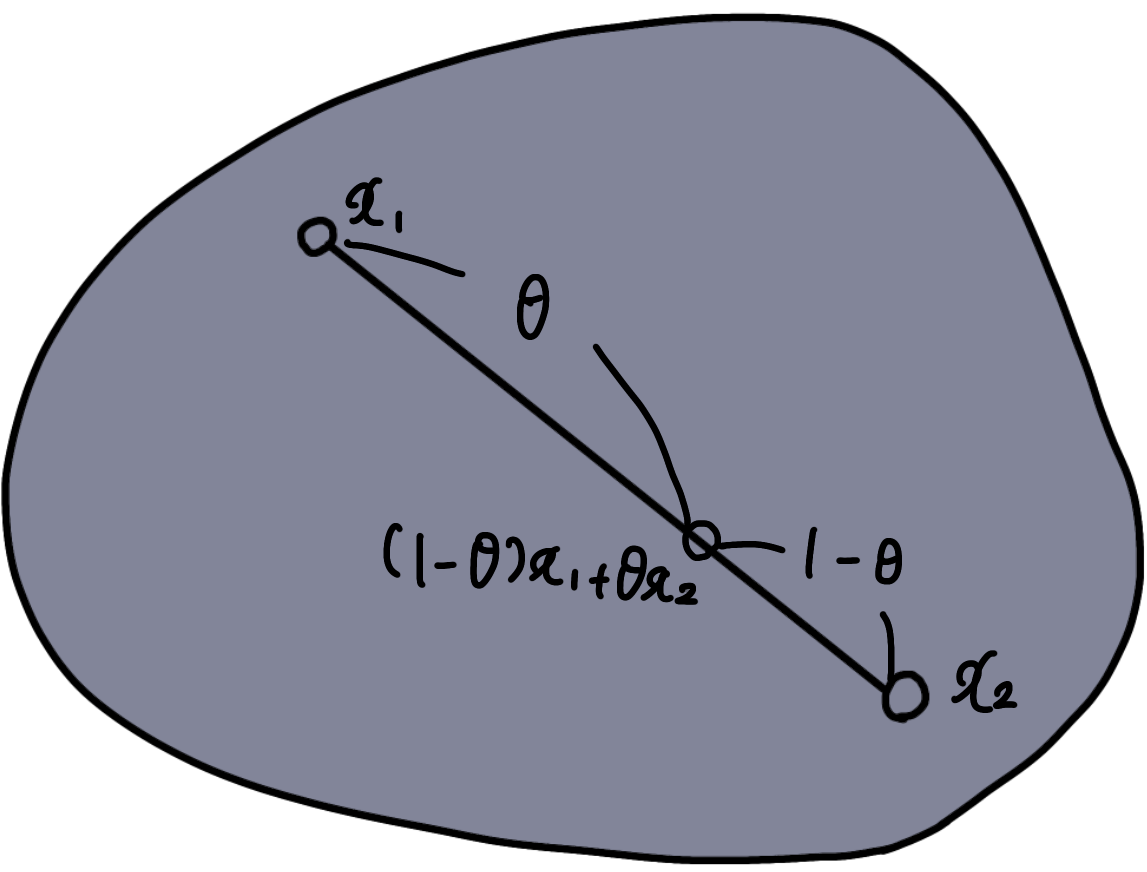
\includegraphics[keepaspectratio, scale=0.12]{convex.png}
			\end{column}
			\begin{column}{0.45\textwidth}
				\centering
				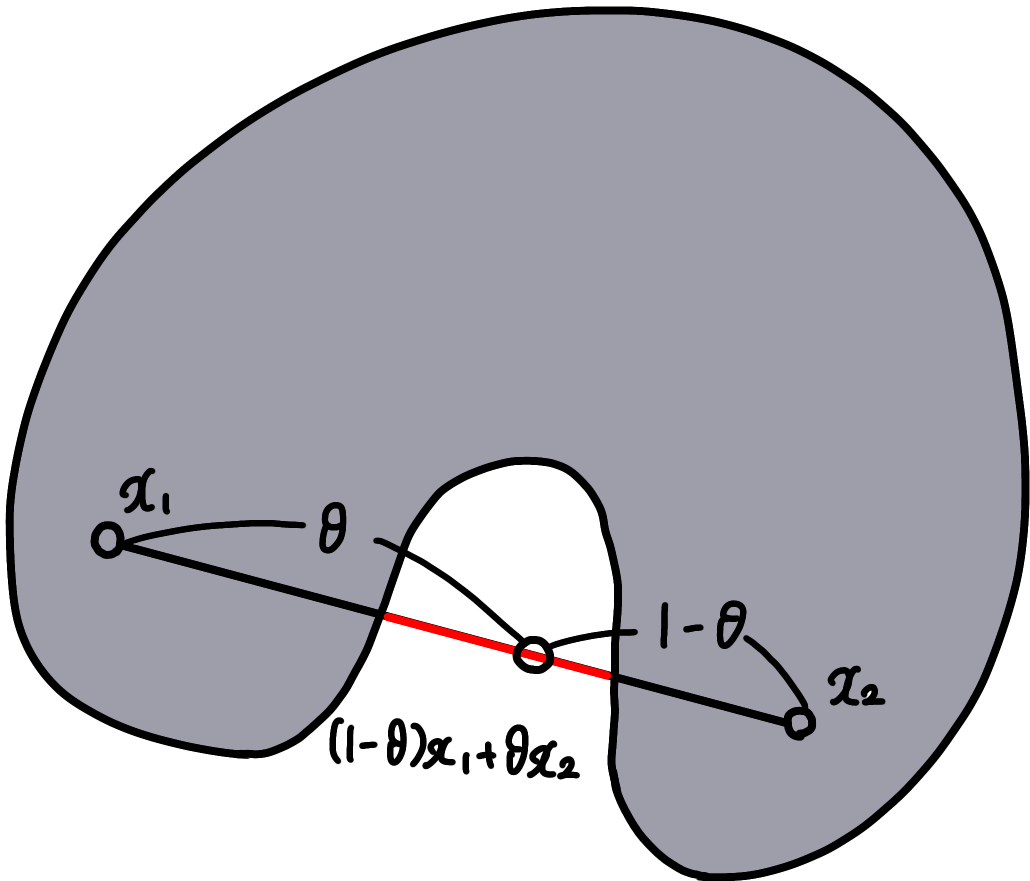
\includegraphics[keepaspectratio, scale=0.12]{non-convex.png}
			\end{column}
		\end{columns}
		\caption{凸集合と非凸集合}
	\end{figure}
\end{frame}


\begin{frame}{凸関数}
    \begin{definition}[凸関数]
        ある実数値関数を$f$とする.$f$のエピグラフが凸集合のとき,$f$は\alert{凸関数}である.
    \end{definition}
    \begin{definition}[エピグラフ]
        以下の集合は,$f$の\alert{エピグラフ}である.
        \begin{align*}
            \epi f \triangleq \left\{(x, y) \in \mathbb{R}^n \times \mathbb{R} : y \geq f(x)\right\}
        \end{align*}
    \end{definition}

    定義の簡単な解釈の仕方としては,
    \begin{itemize}
        \item 関数の上側がエピグラフ
        \item 関数の上側が凹んだりしていなければ,凸関数(下に凸)
    \end{itemize}
\end{frame}

\begin{frame}{凸関数}
    以上2つの定義より,凸関数は一般的に以下のように表される.
    \begin{align}
        (1 - \theta)f(x_1) + \theta f(x_2) \geq f \left( (1 - \theta)x_1 + \theta x_2 \right)
    \end{align}
    % 凸関数と非凸関数の画像を載せる予定
    \begin{figure}[htbp]
		\begin{minipage}[b]{0.45\textwidth}
			\centering
			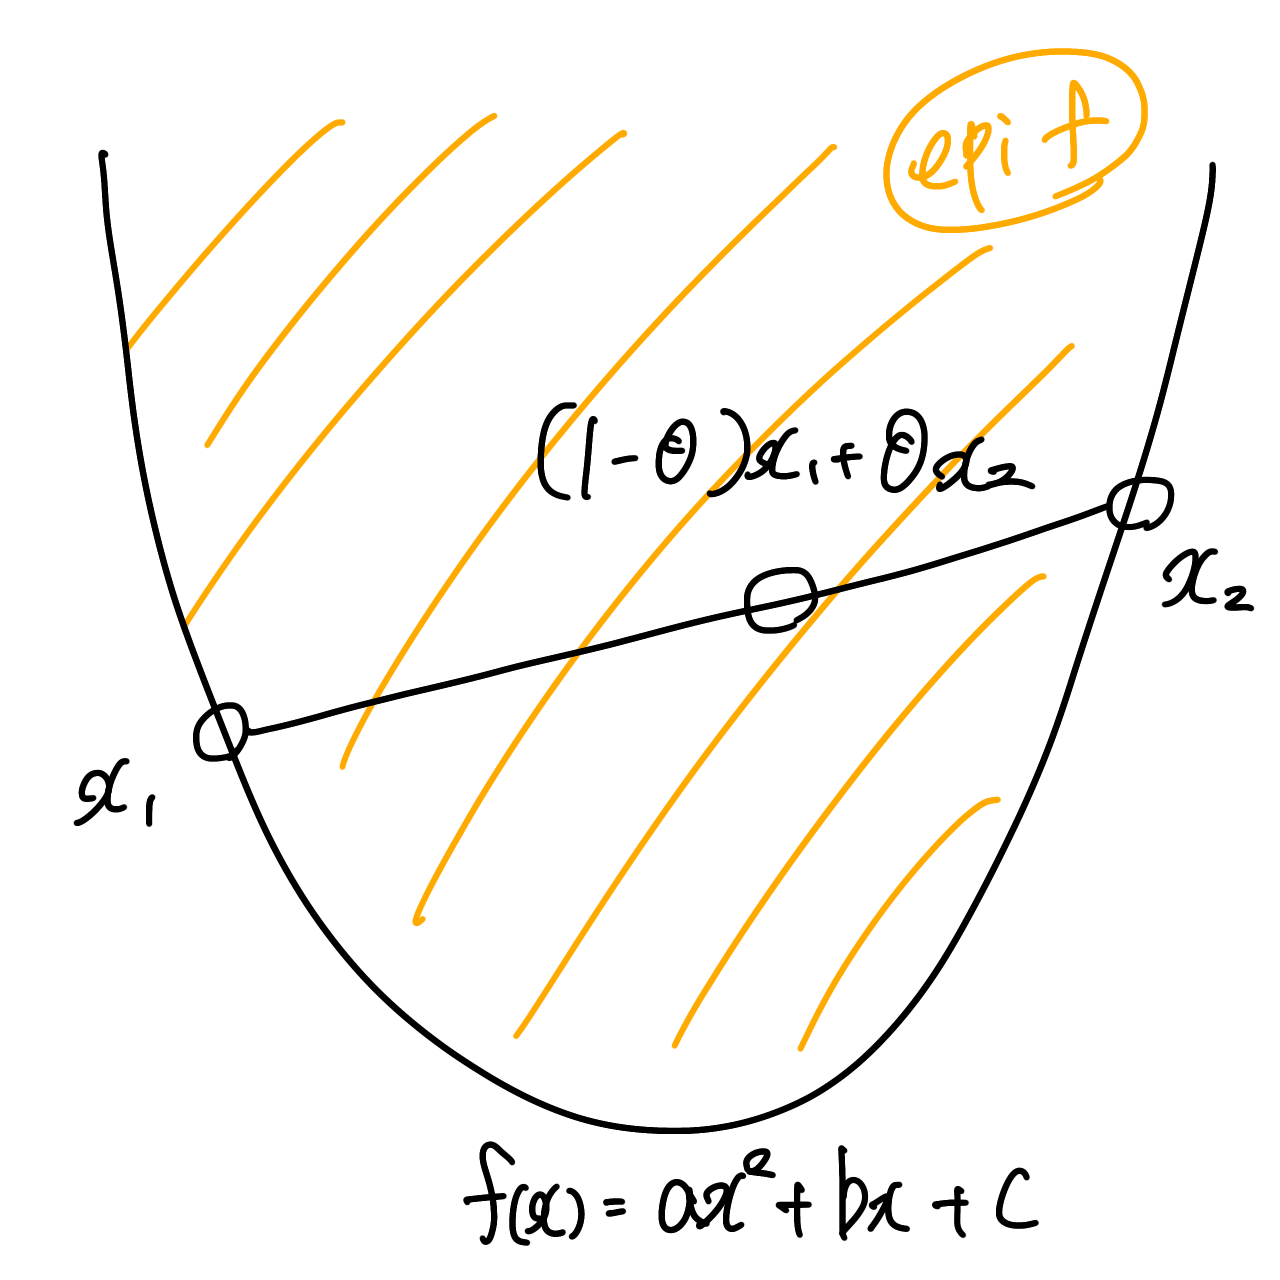
\includegraphics[keepaspectratio, scale=0.12]{convex_function.png}
		\end{minipage}
		\begin{minipage}[b]{0.45\textwidth}
			\centering
			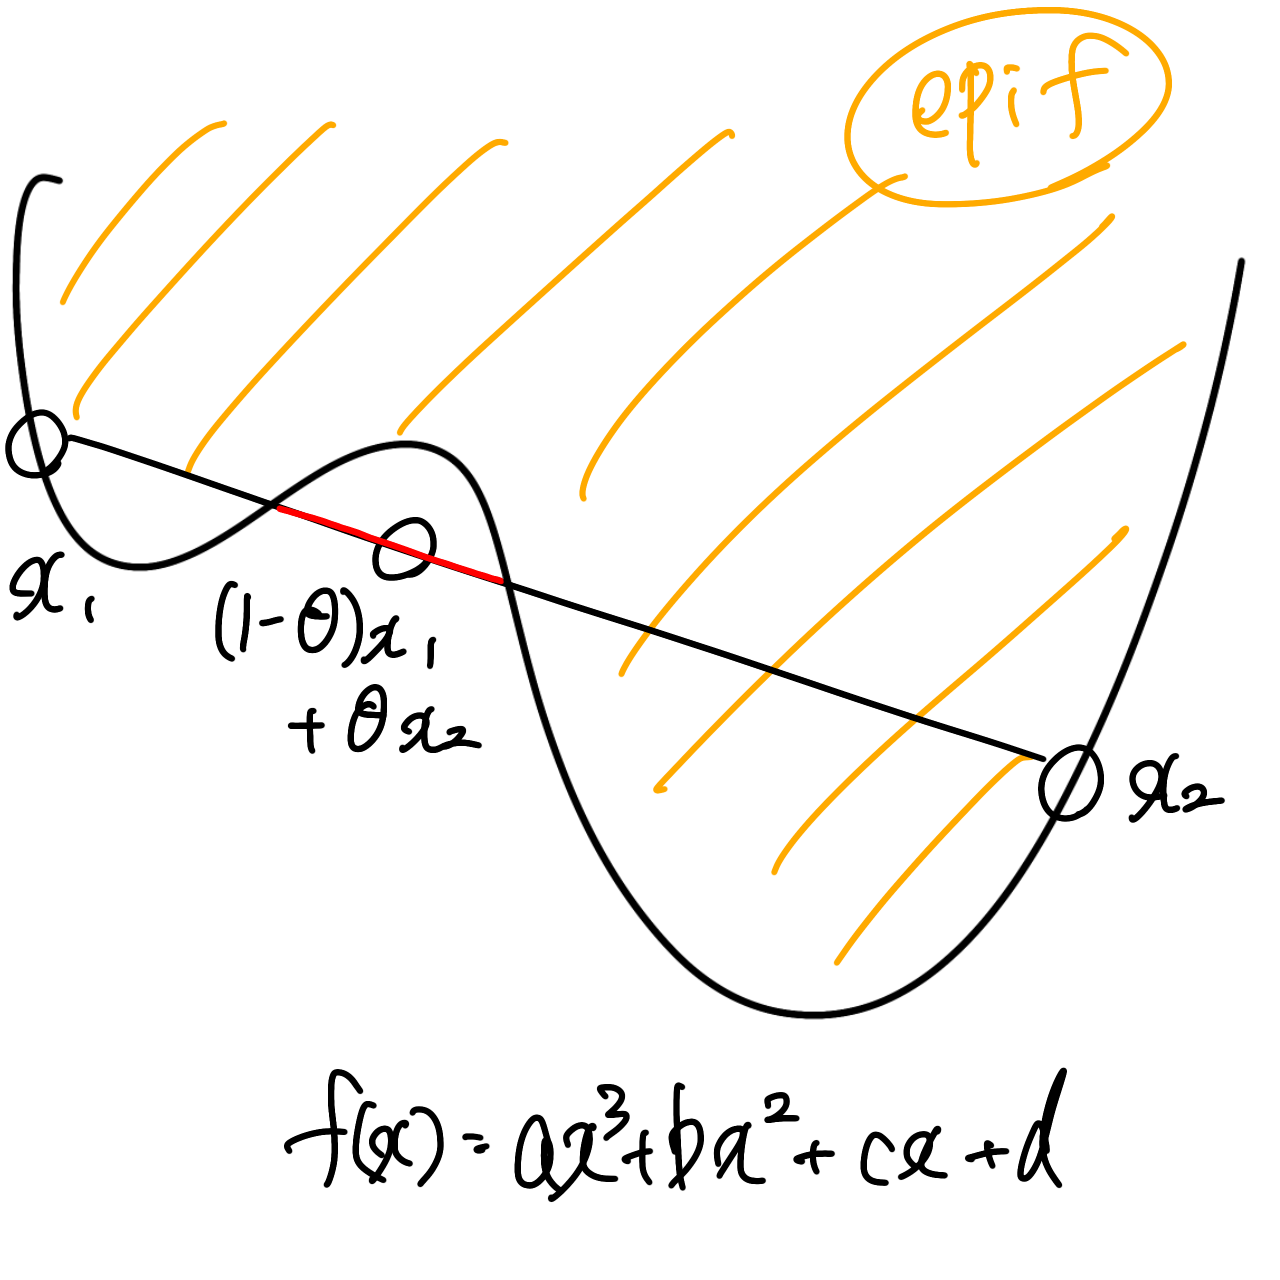
\includegraphics[keepaspectratio, scale=0.12]{non-convex_function.png}
		\end{minipage}
		\caption{凸関数と非凸関数}
	\end{figure}
\end{frame}


\begin{frame}{ちなみに}
    「凸があるなら,凹もあるのでは??」→ あります.えぇ,ありますとも.
    \par
    \par
    \begin{definition}[凹関数]
        ある実数値関数を$g$とする.$g$の符号反転が凸関数である時,$g$は\alert{凹関数}である.  
    \begin{align}
        (1 - \theta)f(x_1) + \theta f(x_2) \leq f \left( (1 - \theta)x_1 + \theta x_2 \right)
    \end{align}
    \end{definition}
    \centering
    \begin{figure}[htbp]
		\begin{minipage}[b]{0.48\textwidth}
			凹関数の例
            \begin{itemize}
                \item 対数関数 $g(x) = \log x$
                \item 正弦関数 $g(x) = \sin x$ ($0 \leq x \leq \pi$)
                \item 二次関数 $g(x) = -x^2$
                \item 平方関数 $g(x) = \sqrt{x}$
            \end{itemize}
    	\end{minipage}
		\begin{minipage}[b]{0.48\textwidth}
			\centering
			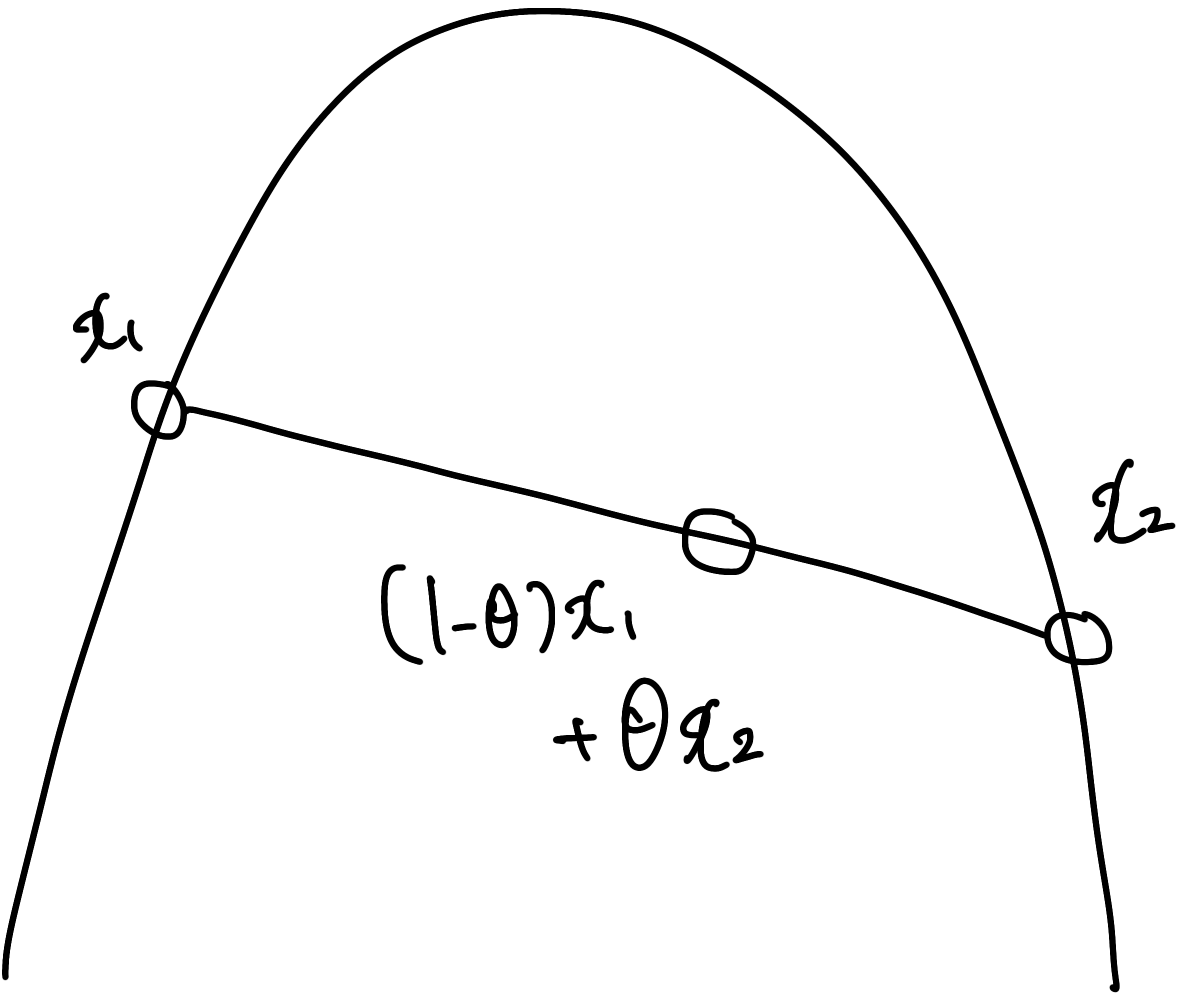
\includegraphics[keepaspectratio, scale=0.1]{concave_function.png}
		\end{minipage}
	\end{figure}
\end{frame}

\section{Convex Optimization}
\begin{frame}{目次}
    \tableofcontents[currentsection]
\end{frame}

\begin{frame}{色んな最適化問題}
    \begin{description}
        \item [線形計画問題]~\\
        目的関数が一次式として表され,制約条件の集合が一次方程式・一次不等式によって定義されている.
        \item [整数計画問題]~\\
        線形計画問題の中で,各変数の値が整数に制限されている問題.
        \item [二次錐計画問題]~\\
        実行可能領域が二次錐(円錐)であるような問題.
        \item [半正定値計画問題]~\\
        半正定値行列を変数とする凸計画問題.
    \end{description}
\end{frame}

\begin{frame}{凸最適化(Convex Optimization)とは}
    \begin{screen}
		関数$f : \mathbb{R}^n \to \mathbb{R} \cup \{ \infty \}$がプロパーな凸関数,かつ集合$C \subset \mathbb{R}^n$が閉凸集合であるとき,$x \subset C$の中で$f(x)$を最小にする$x$を求める問題.
	\end{screen}

    % \vspace{\baselineskip}
    $f(x)<\infty$となるような$x$が一つでも存在する($\dom f \neq \varnothing$)とき,関数$f$はプロパーであるという.
    \begin{definition}[$\dom f$(実効定義域)]
        関数$f$の定義域のうち,$f(x)$が実数値を取るような$x$の集合を\red{$f$の実効定義域}と呼ぶ.
        \begin{align*}
        	\dom f \triangleq \{ x \in \mathbb{R} : f(x) < \infty \}
        \end{align*}
    \end{definition}
\end{frame}

\begin{frame}{凸最適化の何が嬉しいのか}
    \begin{description}
        \item [大域的な最適値を得ることができる]~\\
        一般に,勾配情報を利用した最適化手法では,局所的な最適値に収束することが多い.
        凸最適化では,評価関数の凸性が担保されているため,大域的な最適値を得ることができる.
        \vspace{\baselineskip}
        \item [最適化計算の速度が速い]~\\
        凸最適化特有の最適化手法を用いることで,汎用の最適化手法よりも計算時間を短縮することができる.
        何か,最近では更に高速化を目指した手法があるとかなんとか.
    \end{description}
\end{frame}

\begin{frame}{凸最適化の代表的な手法(アルゴリズム)}
    \begin{itemize}
        \item 最小二乗法
        \item 反復無しニュートン法
        \item 有効制約法
        \item 内点法
        \item 近接勾配法
        \item 交互方向乗数法
    \end{itemize}
\end{frame}

\begin{frame}{アルゴリズムの一例:近接勾配法}
    \begin{screen}
        以下のように定式化される最適化問題を考える.
        \begin{align}
            \label{eq:proximal_gradient_method}
            & && \underset{\omega}{\minimize} && f(\omega) \triangleq g(\omega) + h(\omega) &&
        \end{align}
        ここで,$g$は微分可能な凸関数,$h$は必ずしも微分可能ではない凸関数であるとする.
    \end{screen}
    問題(\ref{eq:proximal_gradient_method})に対する近接勾配法は,以下の更新式によって点$\omega$を更新するアルゴリズムである.
    \begin{align*}
        \omega_{k+1} = \prox_{\gamma h} \left(\omega_k - \gamma \nabla g(\omega_k)\right)
    \end{align*}
    \begin{align*}
       \prox_{\gamma h} (v) \triangleq \argmin_{\omega} \left\{h(\omega) + \frac{1}{2\gamma} \| \omega - v \|_2^2 \right\}
    \end{align*}
    % \begin{align*}
    %     \omega^{(k+1)} \triangleq \argmin_{\omega} \left\{ g(\omega) + \frac{1}{2\alpha} \| \omega - \omega^{(k)} \|_2^2 \right\}
    % \end{align*}
\end{frame}

\begin{frame}{近接勾配法の感覚}
    最速ルートではないけど,それなりに速い(最適解に近い)ルートをたどって進む.
    \begin{figure}
        \centering
        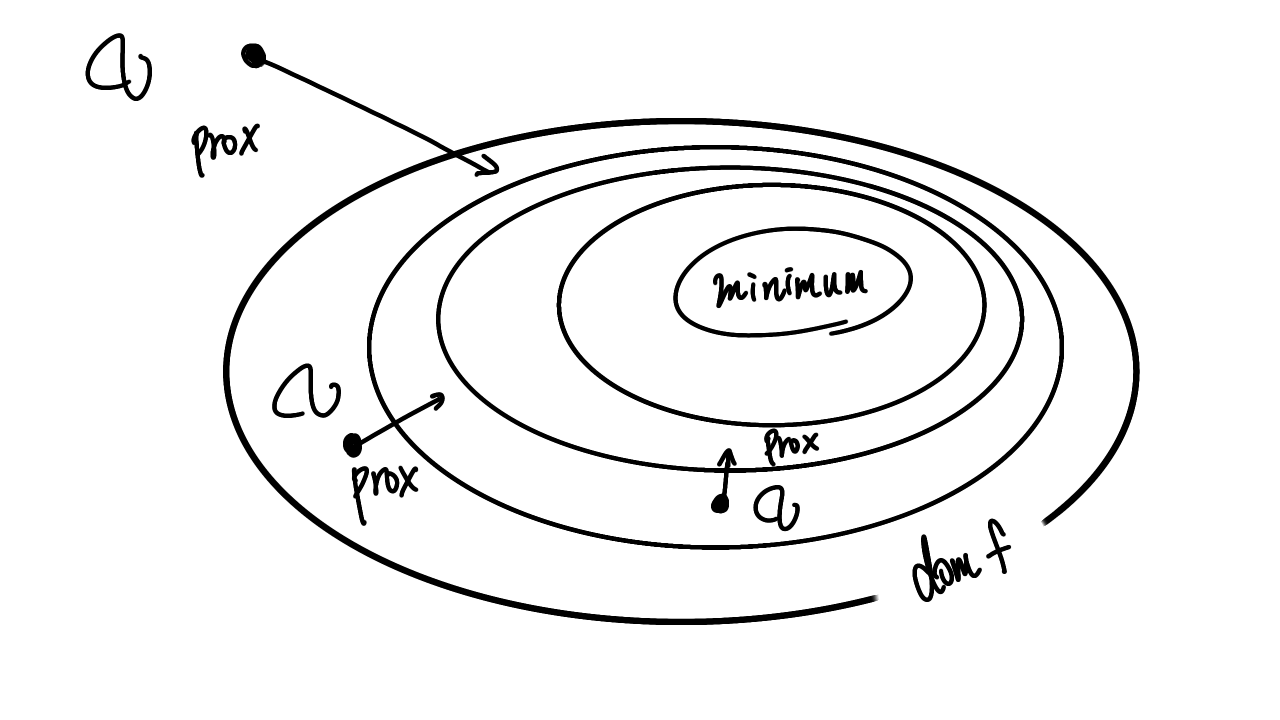
\includegraphics[keepaspectratio, scale=0.2]{prox.png}
        \caption{近接作用素の働き}
    \end{figure}
\end{frame}

\begin{frame}{凸最適化 まとめ}
    \begin{itemize}
        \item 凸最適化とは,目的関数が凸関数で表現される最適化問題のこと.
        \item 凸最適化では,勾配情報を利用しても大域的な最適解を求めれる.
        \item 特有の最適化手法によって,計算を速く行うことができる.
        \begin{itemize}
            \item 最上二乗法
            \item 内点法
            \item 近接勾配法
            \item 交互方向乗数法 などなどetc
        \end{itemize}
    \end{itemize}
\end{frame}

\section{DC Optimization}
\begin{frame}{目次}
	\tableofcontents[currentsection]
\end{frame}

\begin{frame}{DC最適化について}
	\begin{block}{DC最適化とは}
		目的関数が\alert{2つの凸関数の差(Difference of Convex Function)}で表現される非凸最適化問題について,最小化を行う際に使う手法.
	\end{block}
    2つの凸関数$g, h: \mathbb{R}^n \to \mathbb{R} \cup \{ \infty \}$を使って,以下のように表現される.
	\begin{align}
		\label{DCFunc}
		& && \underset{\omega}{\minimize} && g(\omega) - h(\omega) &&
	\end{align}
	\begin{screen}
        関数 $f:\mathbb{R}^n \to \mathbb{R} \cup \{ \infty \}$に対して,2つの閉凸関数$g, h$について
        \begin{align}
            \label{DCFunc2}
            f(\omega) = g(\omega) - h(\omega), \forall \omega \in \mathbb{R}^n
        \end{align}
        が成り立つとき,$f$を\blue{DC関数}といい,(\ref{DCFunc2})の表現を\blue{$f$のDC表現}と呼ぶ.
    \end{screen}
\end{frame}

\begin{frame}{DC最適化について}
    \begin{itembox}[l]{なぜ非凸最適化問題になるのか}
        \begin{itemize}
            \item 凸関数の和は凸関数である.
            \item 凸関数の差は凸関数にならない場合がある.
        \end{itemize}
    \end{itembox}
    凸関数の差を取る最適化問題は一般には非凸最適化問題となり,大局的最適解を求めるのは困難である.\\
    そこで,DCAを用いることで,\red{DC最適化問題を凸最適化問題に変換することができ,凸最適化の手法によって最適解を求めることができる}.\\
    \vspace{\baselineskip}
    なお,2階微分が可能な任意の関数など,多くの関数がDC関数となっている.\\
    → 様々なクラスの最適化問題がDC最適化問題によって表現できる.
\end{frame}

\begin{frame}{DC Algorithm}
    % \begin{figure}
    %     \centering
    %     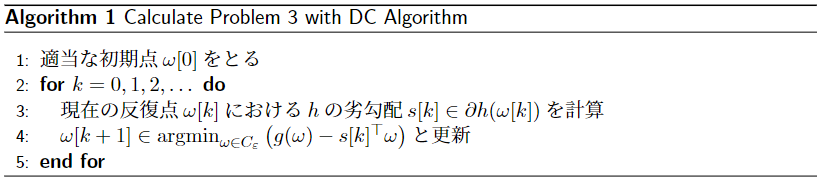
\includegraphics[keepaspectratio, scale=0.8]{DCA.png}
    %     \caption{DCA}
    % \end{figure}
    \begin{algorithm}[H]
        \caption{Calculate Problem (\ref{DCFunc}) with DCA}
        \label{DCA}
        \begin{algorithmic}[1]
            \STATE 適当な初期点$\omega_0$をとる.
            \FOR{$k = 0, 1, 2, \dots$}
            \STATE 現在の反復点$\omega_k$における$h$の劣勾配$s_k \in \partial h(\omega_k)$を計算する.
            \STATE $\omega_{k+1} = \argmin_{\omega} \left(g(\omega) - s_k^{\top} \omega \right)$
            \ENDFOR
        \end{algorithmic}
    \end{algorithm}
    $\partial h(x[k])$:時刻$k$における$x[k]$まわりの劣微分
    \begin{align*}
        \partial h(x[k]) \triangleq \{ s \in \mathbb{R}^n : h(x) \geq h(x[k]) + s^\top (x - x[k]) \}
    \end{align*}
    微分の概念を,微分不可能関数に対しても適用したもの(絶対値関数とか).
\end{frame}

\begin{frame}{DC Algorithmの問題点}
    \begin{align}
        \label{minipro1}
        \omega[k+1] \in \argmin_{\omega}\left(g(\omega) - s[k]^{\top}\omega\right)
    \end{align}
    最適化問題の中に,子問題として凸最適化問題(\ref{minipro1})が含まれており,各反復で(\ref{minipro1})の最適解を求める必要がある.\\

    \red{そのため,大規模な問題や複雑な問題では,莫大な計算コストになる可能性がある}.
    \begin{figure}
        \centering
        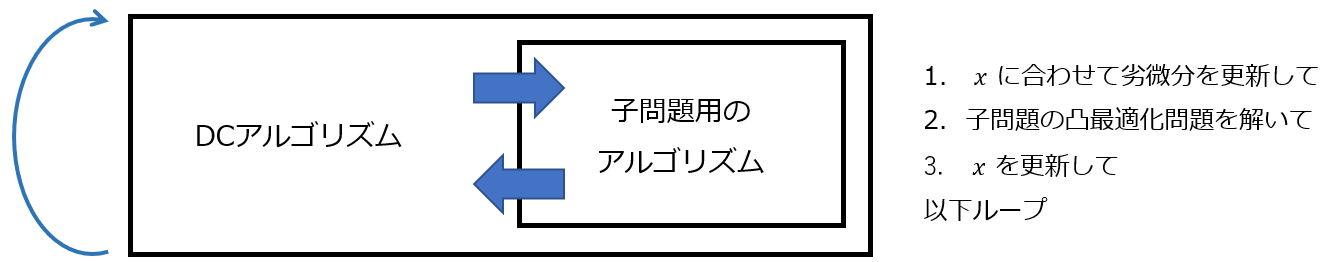
\includegraphics[keepaspectratio, scale=0.4]{DCDC.png}
        \caption{DCAの流れ}
    \end{figure}
\end{frame}

\begin{frame}{pDCA$\varepsilon$}
    最近では問題の構造を活かし,各反復での計算を軽くする手法が提案されている.
    \begin{itembox}[l]{pDCA$\varepsilon$}
        DCAに対して,近接勾配法とNesterovの外挿を施した改良版アルゴリズム.
    \end{itembox}
    % \begin{figure}
    %     \centering
    %     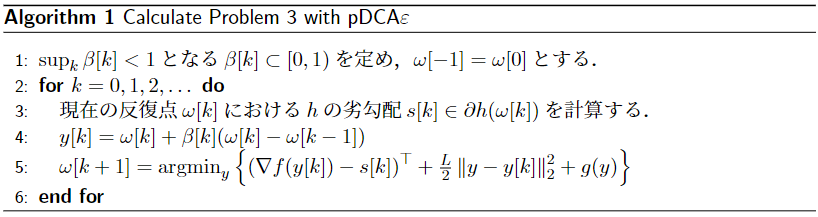
\includegraphics[keepaspectratio, scale=0.8]{pDCAe.png}
    %     \caption{pDCA$\varepsilon$}
    % \end{figure}
    \begin{algorithm}[H]
        \caption{Calculate Problem (\ref{DCFunc}) with pDCA$e$}
        \label{pDCAe}
        \begin{algorithmic}[1]
            \STATE $\sup_{k} \beta_k < 1$となる$\beta_k \subset \left[0, 1\right)$を定め,$\omega_{-1} = \omega_0$とする.
            \FOR{$k = 0, 1, 2, \dots$}
            \STATE 現在の反復点$\omega[k]$における$h$の劣勾配$s_k \in \partial h(\omega_k)$を計算する.
            \STATE $y_k = \omega_k + \beta_k(\omega_k - \omega_{k-1})$
            \STATE $\omega_{k+1} = \argmin_{y} \left\{\left(\nabla f(y_k) - s_k \right)^{\top} + \frac{L}{2} \left\|y-y_k\right\|_{2}^{2} + g(y) \right\}$
            \ENDFOR
        \end{algorithmic}
    \end{algorithm}
\end{frame}

\begin{frame}{凸最適化 まとめ}
    \begin{itemize}
        \item 目的関数が2つの凸関数の差で表現される非凸最適化問題に対する手法.
        \item DCAによって,非凸最適化問題を凸最適化問題に変換することができる.
        \item 多くの関数がDC関数となっていて,様々なクラスの最適化問題をDC最適化問題で表現可能.
        \item ただ,問題によっては大規模な計算コストが必要.
        \item 最近では,計算の軽量化を目指した手法が提案されている.
    \end{itemize}
\end{frame}

\section*{References}
\begin{frame}{References}
    \begin{minipage}[b]{0.95\textwidth}
    {\scriptsize
    \begin{itemize}
        \item 寒野善博, 土谷隆, "東京大学工学教程 基礎系 数学 最適化と変分法", 丸善出版, 2014.
        \item 永原正章, "スパースモデリングー基礎から動的システムの応用ー", コロナ社, 2017.
        \item 伊藤勝, "凸最適化問題に対する一次法とその理論 : 加速勾配法とその周辺", オペレーションズ・リサーチ = Communications of the Operations Research Society of Japan : 経営の科学, 64, 6, pp.326-334, 2019.
        \item 小野峻佑, "近接分離アルゴリズムとその応用: 信号処理・画像処理的観点から", オペレーションズ・リサーチ= Communications of the Operations Research Society of Japan: 経営の科学, 64, 6, pp.316-325, 2019.
        \item 小野峻佑, "近接分離による分散凸最適化―交互方向乗数法に基づくアプローチを中心として―", 計測と制御, 55, 11, pp.954-959, 2016.
        \item 田中未来, 奥野貴之, "DC 最適化の理論と応用", 応用数理, 29, 6, pp.14-23, 2019.
        \item 後藤順哉, 武田朗子, "DC アプローチに基づくスパース最適化", オペレーションズ・リサーチ= Communications of the Operations Research Society of Japan: 経営の科学, 64, 6, pp.352-359, 2019.
        \item Wen, Bo and Chen, Xiaojun and Pong, Ting Kei, "A proximal difference-of-convex algorithm with extrapolation", Computational optimization and applications, 69, pp.297-324, 2018.
    \end{itemize}
    }
\end{minipage}
\end{frame}
% \begin{frame}{ブロック環境}
%     \begin{block}{block}
%     block
%     \end{block}
%     \begin{alertblock}{alertblock}
%     alertblock
%     \end{alertblock}
%     \begin{exampleblock}{exampleblock}
%     exampleblock
%     \end{exampleblock}
%     \begin{tcolorbox}[colframe=green,
%     colback=green!10!white,
%     colbacktitle=green!40!white,
%     coltitle=black, fonttitle=\bfseries,
%     title=My box]
%         box contents
%     \end{tcolorbox}
% \end{frame}

% \section{Section 2}
% \begin{frame}{目次}
%     \tableofcontents[currentsection]
% \end{frame}

% \begin{frame}{箇条書き}
%     \begin{itemize}
%     \item アイテム1
%     \item \alert{アイテム2}
%         \begin{itemize}
%         \item アイテム1
%         \item \alert{アイテム2}
%             \begin{itemize}
%             \item アイテム1
%             \item \alert{アイテム2}
%             \end{itemize}
%         \end{itemize}
%     \end{itemize}
%     \[
%     \bm{x}^\top\bm{y}
%     \]
%     \begin{enumerate}
%     \item abcde
%     \item \structure{ABCDE}
%     \item 
%     \end{enumerate}
% \end{frame}

\end{document}